% ============================================================================
% CHAPTER 2: BASIC CONCEPTS AND LITERATURE REVIEW
% ============================================================================

\chapter{مفاهیم پایه و پیشینه تحقیق}

\section{مقدمه}
از زمان انتشار مشاهده‌های ادوارد لورنز در زمینه‌ی رفتارهای آشوبناک، مفهوم «آشوب» به یکی از موضوعات مورد توجه در جامعه‌ی علمی تبدیل شد. نظریه‌ی آشوب شاخه‌ای از ریاضیات است که به تحلیل سیستم‌هایی می‌پردازد که رفتار آن‌ها به تغییرات کوچک در شرایط اولیه بسیار حساس است. پدیده‌هایی که در مقیاس کوچک آشفته به نظر می‌رسند، ممکن است در مقیاس بزرگ‌تر رفتاری منظم و پایدار داشته باشند.

\section{رمزنگاری}
رمزنگاری (\lr{Cryptography}) از دو واژه‌ی یونانی \lr{krypto} به معنی «پنهان» و \lr{grapho} به معنی «نوشتن» تشکیل شده است.

\subsection{تعریف رمزنگاری}
رمزنگاری فرآیندی است که طی آن اطلاعات به‌گونه‌ای دچار تغییر و بازآرایی می‌شوند که برای افراد غیرمجاز غیرقابل فهم باشد. هدف اصلی رمزنگاری، طراحی طرح‌ها و پروتکل‌هایی است که حتی در حضور دشمن نیز امکان انجام فعالیت‌های خاص را فراهم سازد.

\subsection{شیوه‌های پایه رمزنگاری}
در رمزنگاری کلاسیک، دو شیوه‌ی پایه وجود دارد: جابجایی (\lr{Transposition}) و جایگزینی (\lr{Substitution}).

\subsection{انواع روش‌های رمزنگاری بر اساس نوع کلید}
الگوریتم‌های رمزنگاری به دو دسته متقاران (\lr{Symmetric}) و نامتقاران (\lr{Asymmetric}) تقسیم می‌شوند.

\begin{table}[h]
\centering
\caption{مقایسه رمزنگاری متقارن و نامتقارن}
\begin{tabular}{|l|l|l|}
\hline
\textbf{ویژگی} & \textbf{رمزنگاری متقارن} & \textbf{رمزنگاری نامتقارن} \\ \hline
نوع کلید & یک کلید & یک کلید عمومی و یک کلید خصوصی \\ \hline
نیاز به کانال امن & نیازمند کانال امن & نیاز به کانال امن ندارد \\ \hline
مزیت اصلی & سرعت بالا & امنیت بالا \\ \hline
\end{tabular}
\end{table}

\subsection{ویژگی‌های یک الگوریتم رمزنگاری امن}
یک الگوریتم امن باید دارای ویژگی‌های زیر باشد: یک‌طرفه بودن، عدم وابستگی به الگوریتم (اصل کرشهف)، وابستگی به تمامی بیت‌های کلید و متن اصلی، ساختار جبری پیچیده و برابری طول متن.

\subsection{تحلیل رمز: انواع حملات}
حملات به چهار دسته اصلی تقسیم می‌شوند: حمله با متن رمزشده (\lr{Ciphertext-Only})، حمله با متن اصلی مشخص (\lr{Known-Plaintext})، حمله با متن اصلی منتخب (\lr{Chosen-Plaintext}) و حمله با متن رمزشده منتخب (\lr{Chosen-Ciphertext}).

\subsection{امنیت سیستم‌های رمزنگاری}
\subsubsection{اصول شش‌گانه کرشهف}
آگوست کرشهف در سال ۱۸۸۳ اصول اساسی را مطرح کرد که مهم‌ترین آن‌ها محرمانه بودن تنها کلید رمز است.

\subsubsection{معیارهای پنجگانه شانون}
کلاد شانون در سال ۱۹۴۸ معیارهای پنجگانه‌ای شامل میزان ایمنی، اندازه کلید، پیچیدگی عملیات، انتشار خطا و بسط پیام را معرفی نمود.

\section{رمزنگاری تصویر دیجیتال}
تصاویر دیجیتال به دلیل حجم بالا و همبستگی شدید پیکسل‌های مجاور، نیازمند الگوریتم‌های اختصاصی هستند. روش‌هایی مانند \lr{AES} و \lr{RSA} برای تصاویر کارا نیستند.

\section{نظریه‌ی آشوب و مفاهیم بنیادی آن}
نظریه آشوب با پژوهش‌های ادوارد لورنز و کشف «اثر پروانه‌ای» به اوج رسید. 

\begin{figure}[h]
    \centering
    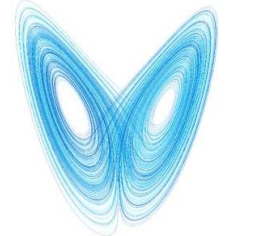
\includegraphics[width=0.4\textwidth]{vertopal_6a6e478acc1947c1bfecfac3523ed62b/media/image2}
    \caption{اثر پروانه‌ای و حساسیت به شرایط اولیه}
\end{figure}

\subsection{ویژگی‌های تئوری آشوب}
\begin{itemize}
    \item \textbf{اثر پروانه‌ای:} حساسیت شدید به شرایط اولیه.
    \item \textbf{سازگاری پویا:} توانایی تطبیق با محیط.
    \item \textbf{جذب‌کننده عجیب:} ساختارهای پیچیده فراکتالی.
    \item \textbf{خودتشابهی:} تکرار الگوها در مقیاس‌های مختلف.
\end{itemize}

\subsection{نمونه‌هایی از سیستم‌های آشوبی}

\subsubsection{نگاشت لجستیک}
این نگاشت یک‌بعدی با رابطه زیر تعریف می‌شود:
\begin{equation}
    x_{n+1} = r x_n (1-x_n)
\end{equation}
\begin{figure}[h]
    \centering
    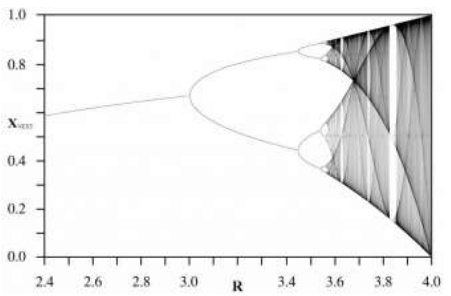
\includegraphics[width=0.5\textwidth]{vertopal_6a6e478acc1947c1bfecfac3523ed62b/media/image4}
    \caption{نمودار دوشاخگی نگاشت لجستیک}
\end{figure}

\subsubsection{سیستم آشوبی لورنز}
این سیستم سه‌بعدی برای مدل‌سازی جو ارائه شده است:
\begin{figure}[h]
    \centering
    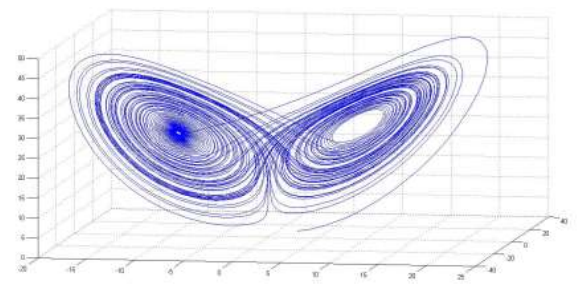
\includegraphics[width=0.4\textwidth]{vertopal_6a6e478acc1947c1bfecfac3523ed62b/media/image7}
    \caption{جذب‌کننده عجیب لورنز}
\end{figure}

\subsubsection{سیستم آشوبی چن}
این سیستم پیچیدگی بالاتری نسبت به لورنز دارد:
\begin{figure}[h]
    \centering
    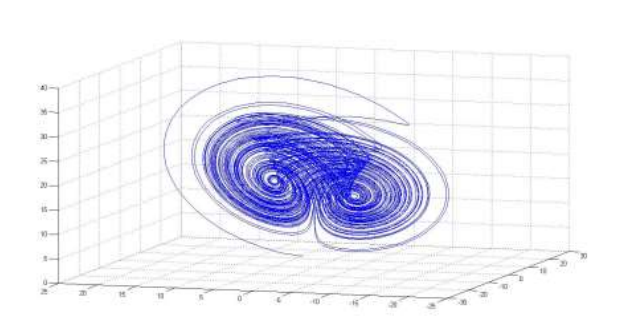
\includegraphics[width=0.5\textwidth]{vertopal_6a6e478acc1947c1bfecfac3523ed62b/media/image9}
    \caption{نمای سه‌بعدی سیستم آشوبی چن}
\end{figure}

\section{ارتباط بین آشوب و رمزنگاری}
شباهت‌های ساختاری میان این دو سیستم در جدول زیر خلاصه شده است:

\begin{table}[h]
\centering
\caption{شباهت‌های سیستم‌های رمز متداول و سیستم‌های آشوبناک}
\begin{tabular}{|l|l|}
\hline
\textbf{سیستم‌های رمز متداول} & \textbf{سیستم‌های آشوبناک} \\ \hline
اغتشاش (\lr{Confusion}) & اغتشاش (\lr{Ergodicity}) \\ \hline
انتشار (\lr{Diffusion}) & حساسیت به شرایط اولیه \\ \hline
کلید رمز & شرایط اولیه و پارامترها \\ \hline
دور (\lr{Cycle}) & تکرار \\ \hline
\end{tabular}
\end{table}

\section{پیشینه پژوهش}
پژوهش‌های ژانگ و لیو (۲۰۲۳)، هو و ژو (۲۰۱۹) و خدادادی و زندوکیلی (۲۰۱۹) مبانی استفاده از سیستم‌های آشوبی ترکیبی در امنیت تصاویر رنگی را بنا نهاده‌اند.
\
